\chapter{Project: Tối ưu Phí Gas Ethereum bằng Offline Reinforcement Learning}

% ============================================================
\section{Lý thuyết Nền tảng}
% ============================================================

\subsection{Markov Decision Process (MDP)}

Bài toán điều phối giao dịch được mô hình hóa dưới dạng \textbf{Markov Decision Process} (MDP), được định nghĩa bởi bộ $(\mathcal{S}, \mathcal{A}, P, R, \gamma)$:

\begin{itemize}
    \item $\mathcal{S}$: Không gian trạng thái — mô tả trạng thái hiện tại của hệ thống.
    \item $\mathcal{A}$: Không gian hành động — tập các quyết định có thể thực hiện.
    \item $P(s' | s, a)$: Hàm chuyển trạng thái — xác suất chuyển sang $s'$ khi ở $s$ thực hiện $a$.
    \item $R(s, a)$: Hàm phần thưởng — tín hiệu phản hồi từ môi trường.
    \item $\gamma \in [0,1)$: Hệ số chiết khấu tương lai.
\end{itemize}

Mục tiêu là tìm chính sách (policy) $\pi: \mathcal{S} \to \mathcal{A}$ tối đa hóa tổng phần thưởng kỳ vọng chiết khấu:
\begin{equation}
    J(\pi) = \mathbb{E}_\pi\left[\sum_{t=0}^{\infty} \gamma^t R(s_t, a_t)\right]
\end{equation}
Đây chính là nền tảng để xây dựng bài toán RL nơi mà Dữ liệu/Môi trường phải đưa về dạng có $\mathcal{S}$ (state) và $\mathcal{A}$ (action).

\subsection{Q-Learning và Phương trình Bellman}

\textbf{Q-function} (hay Action-Value function) $Q^\pi(s, a)$ biểu diễn tổng phần thưởng kỳ vọng khi ở trạng thái $s$, thực hiện hành động $a$, và sau đó tuân theo chính sách $\pi$:
\begin{equation}
    Q^\pi(s, a) = \mathbb{E}_\pi\left[\sum_{k=0}^{\infty} \gamma^k R(s_{t+k}, a_{t+k}) \;\Big|\; s_t = s, a_t = a\right]
\end{equation}

Phương trình Bellman biểu diễn tính nhất quán đệ quy của $Q$-function:
\begin{equation}
    Q^\pi(s, a) = R(s, a) + \gamma \sum_{s'} P(s'|s,a)\, Q^\pi(s', \pi(s'))
    \label{eq:bellman}
\end{equation}

Q-function tối ưu $Q^*(s,a) = \max_\pi Q^\pi(s,a)$ thỏa:
\begin{equation}
    Q^*(s, a) = R(s, a) + \gamma \sum_{s'} P(s'|s,a) \max_{a'} Q^*(s', a')
\end{equation}

Chính sách tối ưu: $\pi^*(s) = \arg\max_a Q^*(s, a)$.

\subsection{Offline Reinforcement Learning}

Trong \textbf{Online RL}, agent học bằng cách tương tác trực tiếp với môi trường — mỗi hành động tạo ra dữ liệu mới. Trong \textbf{Offline RL} \cite{levine2020offline}, agent chỉ được học từ tập dữ liệu lịch sử cố định:
\begin{equation}
    \mathcal{D} = \{(s_i, a_i, r_i, s'_i)\}_{i=1}^{N}
\end{equation}
thu thập bởi một chính sách hành vi (behavior policy) $\pi_\beta$ — không nhất thiết là tối ưu.

\textbf{Thách thức cốt lõi}: \textit{Distribution shift} hay \textit{Extrapolation Error}. Khi agent muốn đánh giá Q-value của một hành động $a_{\text{OOD}} \notin \mathcal{D}$, mạng $Q_\theta$ được huấn luyện bằng dữ liệu từ $\pi_\beta$ sẽ \textit{extrapolate} không chính xác và thường overestimate $Q_\theta(s, a_{\text{OOD}})$. Điều này dẫn đến policy chọn các hành động "ảo tưởng" không có trong data, gây sụp đổ.

\subsection{Conservative Q-Learning (CQL)}

\textbf{Discrete CQL} \cite{kumar2020conservative} giải quyết extrapolation error bằng cách thêm một \textit{conservative penalty} trực tiếp vào hàm mục tiêu huấn luyện:

\begin{equation}
    \mathcal{L}_{\text{CQL}}(\theta) = \underbrace{\mathbb{E}_{(s,a,r,s')\sim\mathcal{D}}\left[(Q_\theta(s,a) - y)^2\right]}_{\mathcal{L}_\text{TD} \text{ — Bellman Error}} 
    + \alpha \underbrace{\mathbb{E}_{s\sim\mathcal{D}}\left[\log\sum_{a'} e^{Q_\theta(s,a')} - \mathbb{E}_{a\sim\pi_\beta}[Q_\theta(s,a)]\right]}_{\text{Conservative Penalty}}
    \label{eq:cql}
\end{equation}

Trong đó $y = r + \gamma \max_{a'} Q_{\bar\theta}(s', a')$ là Bellman target (dùng target network $\bar\theta$).

\textbf{Ý nghĩa hình học của Conservative Penalty:}
\begin{itemize}
    \item Số hạng $\log\sum_{a'} e^{Q_\theta(s,a')}$: \textit{softmax} của tất cả Q-values → tác động như lực kéo xuống đều lên mọi hành động.
    \item Số hạng $\mathbb{E}_{a\sim\pi_\beta}[Q_\theta(s,a)]$: lực đẩy lên đối với các hành động có trong data.
    \item Hiệu số: Q-values của OOD actions bị hạ thấp, Q-values của in-distribution actions được nâng cao.
\end{itemize}

Kết quả: policy học được sẽ ưa thích các hành động đã được quan sát trong $\mathcal{D}$ — đặc biệt là những hành động từ Oracle có reward cao.

\subsection{Quy hoạch Động (Dynamic Programming)}

\textbf{Backward Induction} là phương pháp DP tìm chính sách tối ưu \textit{toàn cục} trong bài toán hữu hạn bước $T$. Thuật toán bắt đầu từ bước cuối và tính ngược về bước đầu:

\textbf{Khởi tạo:} $V[T, Q] = $ chi phí tối thiểu khi chỉ còn $Q$ giao dịch và đã hết thời gian.

\textbf{Bước quy hoạch} (với $t = T-1, T-2, \ldots, 0$):
\begin{equation}
    V[t, Q] = \min_{b \in \mathcal{A}}\; \left\{c(t, Q, b) + V[t+1, f(Q, b, t)]\right\}
    \label{eq:dp}
\end{equation}

Trong đó:
\begin{itemize}
    \item $c(t, Q, b)$: chi phí tức thời khi ở $(t, Q)$ chọn bin $b$ — gồm gas cost và urgency penalty.
    \item $f(Q, b, t) = \max(0, Q - n_b) + w_{t+1}$: hàm chuyển trạng thái queue.
\end{itemize}

DP đảm bảo kết quả là \textbf{optimal global strategy} vì nó xét \textit{toàn bộ} quỹ đạo tương lai có thể xảy ra.

% ============================================================
\section{Phát biểu Bài toán}
% ============================================================

\subsection{Mô hình hóa Bài toán Điều phối Giao dịch}

Xét một tổ chức cần xử lý $Q_0$ giao dịch trên Ethereum trong khoảng thời gian $[0, T]$ ($T = 24$ giờ). Tại mỗi block (bước thời gian $t$), hệ thống phải quyết định số lượng giao dịch cần gửi.

\textbf{MDP của bài toán:}
\begin{itemize}
    \item \textbf{State:} $s_t = (g_t, g_{t-1}, g_{t-2}, p_t, m_t, a_t, u_t, b_t, Q_t, \tau_t, \bar{g}_t) \in \mathbb{R}^{11}$
    \item \textbf{Action:} $a_t \in \{0, 1, 2, 3, 4\}$ — bin ID tương ứng tỷ lệ xả $\{0\%, 25\%, 50\%, 75\%, 100\%\}$
    \item \textbf{Transition:} $Q_{t+1} = \max(0, Q_t - n_t) + w_{t+1}$
    \item \textbf{Reward:} $r_t$ được thiết kế để tối thiểu hóa chi phí gas và phạt deadline
    \item \textbf{Horizon:} $T = 24$ giờ (1 episode = 1 ngày)
\end{itemize}

\textbf{Bài toán tối ưu:}
\begin{equation}
    \min_{\pi} \mathbb{E}\left[\sum_{t=0}^{T-1} \frac{g_t}{\sigma}\left(C_{\text{base}}\cdot\mathbf{1}[n_t>0] + C_{\text{mar}}\cdot n_t\right) + \frac{\lambda}{\sigma}\cdot\mathbf{1}[Q_T > 0]\right]
    \label{eq:objective}
\end{equation}

\subsection{Ánh xạ Dữ liệu Chuỗi thời gian thành Bộ Transitions MDP}

Trong thực tế, dữ liệu thu thập từ blockchain Ethereum là dữ liệu chuỗi thời gian (time-series) thô. Để áp dụng Offline RL, ta phải biến đổi các log dữ liệu này thành tập các bộ chuyển trạng thái (Transitions) $\mathcal{D} = \{(s_t, a_t, r_t, s_{t+1})\}$. Quy trình ánh xạ từ dữ liệu thô sang các thành phần của MDP được thực hiện như sau:

\begin{enumerate}
    \item \textbf{Khởi tạo Trạng thái ($s_t \in \mathcal{S}$):} 
    Tại mỗi block $t$, từ các dữ liệu thô như giá gas và số lượng giao dịch, ta áp dụng Feature Engineering để tính toán ra vector 11 chiều (đã mô tả ở Bảng \ref{tab:state}). Vector này đóng vai trò là $s_t$, đại diện đầy đủ cho môi trường tại block đó.
    
    \item \textbf{Xác định Hành động ($a_t \in \mathcal{A}$):} 
    Dữ liệu thô chỉ ghi nhận số lượng transaction được bot cũ xử lý. Ta lấy số lượng đó chia cho dung lượng tối đa của một block để ra một tỷ lệ liên tục $[0, 1]$. Sau đó, ta lượng hóa tỷ lệ này thành 5 nhãn rời rạc $\{0, 1, 2, 3, 4\}$ tương ứng với các bin $\{0\%, 25\%, 50\%, 75\%, 100\%\}$ để làm hành động $a_t$.
    
    \item \textbf{Mô phỏng Chuyển trạng thái ($P(s_{t+1}|s_t, a_t)$):} 
    Vì đây là Offline RL, ta không có môi trường thật để tương tác sinh ra $s_{t+1}$. Ta giải quyết bằng cách áp dụng \textbf{Mô hình vật lý của Hàng đợi}:
    $$Q_{t+1} = \max(0, Q_t - n_t) + w_{t+1}$$
    Trong đó $n_t$ là số giao dịch thực thi (phụ thuộc vào $a_t$) và $w_{t+1}$ là số giao dịch mới đổ vào block sau (lấy từ dữ liệu lịch sử). Nhờ vậy, ta tự tạo ra được trạng thái tiếp theo $s_{t+1}$ đảm bảo tính nhất quán về mặt nhân quả (Causal Consistency).
    
    \item \textbf{Tính toán Phần thưởng ($R(s_t, a_t)$):} 
    Dựa vào trạng thái $s_t$ và hành động $a_t$ vừa xác định, ta áp dụng hàm toán học đã thiết kế (Phương trình 2.12) để tính ra một con số cụ thể cho $r_t$.
\end{enumerate}

Kết quả của quá trình này là từ một bảng dữ liệu thô không có cấu trúc RL, ta thu được một tập dữ liệu chuẩn MDP $\mathcal{D} = \{(s_t, a_t, r_t, s_{t+1})\}_{t=1}^{N}$ sẵn sàng nạp vào thuật toán Discrete CQL để huấn luyện.

\subsection{Không gian Trạng thái — 11 Chiều}

\begin{table}[ht]
\centering
\caption{Thiết kế Vector Trạng thái $s_t \in \mathbb{R}^{11}$}
\begin{tabular}{clp{7.5cm}}
\hline
\textbf{Idx} & \textbf{Ký hiệu} & \textbf{Công thức / Ý nghĩa} \\
\hline
0--2 & $g_t, g_{t-1}, g_{t-2}$ & Lịch sử giá gas (gas price, wei) — 3 block gần nhất \\
3    & $p_t$                   & Tắc nghẽn mạng: $(gas\_used_t - target_t)/target_t$ \\
4    & $m_t$                   & Momentum giá: $\log(g_t) - \log(g_{t-1})$ \\
5    & $a_t$                   & Acceleration: $m_t - m_{t-1}$ \\
6    & $u_t$                   & Transaction surprise: $(tx_t - \mu_{tx})/\sigma_{tx}$ \\
7    & $b_t$                   & Backlog pressure: $\rho b_{t-1} + \alpha_b p_t + \beta_b u_t$ \\
8    & $Q_t$                   & Kích thước hàng đợi hiện tại (số giao dịch) \\
9    & $\tau_t$                & Thời gian còn lại đến deadline (giờ) \\
10   & $\bar{g}_t$             & Giá gas tham chiếu: trung bình trượt 128 block \\
\hline
\end{tabular}
\label{tab:state}
\end{table}

\textbf{Thiết kế đặc biệt:} $b_t$ (Backlog Pressure) là chỉ số tích lũy theo thời gian, bắt chước "áp lực tắc nghẽn tích luỹ" thực tế trên mạng. Công thức: $b_t = \max(0, \rho\cdot b_{t-1} + \alpha_b\cdot p_t + \beta_b\cdot u_t)$ với $\rho=0.95$, $\alpha_b=0.3$, $\beta_b=0.2$.

\subsection{Không gian Hành động Rời rạc}

\begin{equation}
    \mathcal{A} = \{0, 1, 2, 3, 4\}\;\; \leftrightarrow \;\; r(a) \in \{0\%, 25\%, 50\%, 75\%, 100\%\}
\end{equation}

Số giao dịch thực thi: $n_t = \min\!\left(\!\lfloor r(a_t)\cdot Q_t \rceil, C_{\text{cap}}\right)$ với $C_{\text{cap}} = 500$.

\textbf{Lý do sử dụng không gian rời rạc:} Trong thực nghiệm với IQL liên tục, phân phối hành động trong dataset có cấu trúc đa đỉnh tại $\{0, 0.5, 1\}$. Gaussian Actor (dùng trong IQL) không thể fit phân phối này, luôn hội tụ về $\bar{a}\approx 0.46$ — dẫn đến policy collapse hoàn toàn (deadline miss rate = 100\%).

Chuyển sang không gian rời rạc biến bài toán \textit{hồi quy liên tục} thành bài toán \textit{phân loại} — phù hợp hơn với cấu trúc dữ liệu thực tế.

\subsection{Hàm Phần thưởng}

Phần thưởng tại mỗi bước $t$ gồm 3 thành phần:
\begin{equation}
    r_t = \underbrace{-\frac{g_t}{\sigma}\!\left(C_{\text{base}}\cdot\mathbf{1}[n_t>0] + C_{\text{mar}}\cdot n_t\right)}_{\text{(1) Chi phí gas}} \;-\; \underbrace{\frac{\beta}{\sigma}\cdot Q_{\text{remain}}\cdot e^{\alpha(1-\tau_t)}}_{\text{(2) Urgency (mũ)}}\; -\; \underbrace{\frac{\lambda}{\sigma}\cdot\mathbf{1}[Q_T > 0]}_{\text{(3) Deadline penalty}}
    \label{eq:reward}
\end{equation}

Tham số: $C_{\text{base}}=21{,}000$, $C_{\text{mar}}=15{,}000$ (gas units); $\beta=100$ (urgency weight); $\alpha=3.0$ (urgency exponent); $\lambda=5\times10^9$ (deadline penalty); $\sigma=10^9$ (reward scale).

\textbf{Thiết kế thành phần (2) — Urgency penalty:} Hàm mũ $e^{\alpha(1-\tau_t)}$ tăng nhanh khi $\tau_t\to 0$. Khi còn nhiều thời gian ($\tau_t\approx 1$), penalty nhỏ — agent có thể "chờ" giá gas rẻ hơn. Khi gần deadline ($\tau_t\approx 0$), penalty lớn — agent bị áp lực phải xả giao dịch dù giá cao.

% ============================================================
\section{Triển khai Hệ thống}
% ============================================================

\subsection{Hindsight Oracle — Bộ Giải Tối ưu Toàn cục}

\subsubsection{Động lực}

Dataset thô chứa hành vi của người vận hành (behavior policy $\pi_\beta$) — thường là suboptimal. Để CQL học được chiến lược vượt trội, ta cần dữ liệu "chuyên gia". Thay vì dùng human expert, ta xây dựng \textbf{Hindsight Oracle}: một bộ giải DP \textit{toàn tri} — biết trước giá gas của toàn bộ 24h — để tạo ra quỹ đạo tối ưu làm nhãn huấn luyện.

\subsubsection{Thuật toán DP Solver}

Oracle giải phương trình DP (\ref{eq:dp}) trên không gian trạng thái $(t, Q)$:

\paragraph{Bước 1 — Backward pass (tính value table):}
\begin{align}
    V[T,Q] &= \min_{b\in\mathcal{A}} c(T, Q, b) \quad\quad\text{(không có tương lai)} \\
    V[t,Q] &= \min_{b\in\mathcal{A}} \left\{c(t, Q, b) + V[t+1, f(Q,b,t)]\right\} \quad t = T-1,\ldots,0
\end{align}

Chi phí tức thời cho bin $b$ tại $(t, Q)$:
\begin{equation}
    c(t,Q,b) = \frac{g_t}{\sigma}\!\left(C_{\text{base}}\!\cdot\!\mathbf{1}[n_b>0] + C_{\text{mar}}\!\cdot\! n_b\right) + \frac{\beta}{\sigma}\cdot(Q-n_b)\cdot e^{\alpha(1-\tau_t)}
\end{equation}

\paragraph{Bước 2 — Forward tracing (lấy quỹ đạo tối ưu):}
\begin{equation}
    a^*_t = \arg\min_{b\in\mathcal{A}} \left\{c(t, Q_t, b) + V[t+1, f(Q_t, b, t)]\right\}
\end{equation}

Từ $t=0$ đến $t=T-1$, theo vết chính sách $\text{Policy}[t,Q]$ đã ghi trong backward pass.

\paragraph{Độ phức tạp:}
\begin{itemize}
    \item Discrete Oracle: $O(Q_{\max}\cdot T\cdot|\mathcal{A}|) = O(Q_{\max}\cdot T\cdot 5)$
    \item Continuous Oracle (cũ): $O(Q_{\max}\cdot T\cdot C_{\text{cap}}) = O(Q_{\max}\cdot T\cdot 500)$
\end{itemize}

Giảm $100\times$ số phép tính, đồng thời loại bỏ sai lệch lượng hóa (quantization error).

\subsubsection{Cài đặt — Numba JIT}

DP solver được biên dịch bằng \texttt{@njit(cache=True)} của Numba. Kết hợp với \texttt{ProcessPoolExecutor}, các episode được xử lý song song, đạt tốc độ nhanh hơn Python thuần $\approx100\times$:

\begin{lstlisting}[style=PythonStyle, caption={Vòng lặp DP lõi (pseudo-code Numba JIT)}]
@njit(cache=True)
def _compute_trajectory_njit(gas_prices, incoming_requests, Q_max, ...):
    # Bước 1: Backward pass
    V = np.full((T+1, Q_max+1), INF)
    Policy = np.zeros((T, Q_max+1), dtype=int64)
    for t in range(T-1, -1, -1):
        for Q in range(Q_max+1):
            best_cost = INF
            for b in range(5):  # 5 discrete bins
                ratio = bins[b]
                n = min(int(ratio * Q), cap)
                cost = gas_cost(t, n) + urgency_cost(t, Q-n) + V[t+1, Q_next(Q,n,t)]
                if cost < best_cost:
                    best_cost = cost
                    Policy[t, Q] = b
            V[t, Q] = best_cost
    # Bước 2: Forward trace
    return forward_trace(Policy, Q_init, arrivals)
\end{lstlisting}

\subsection{Pipeline Xây dựng Dataset}

\begin{figure}[ht]
\centering
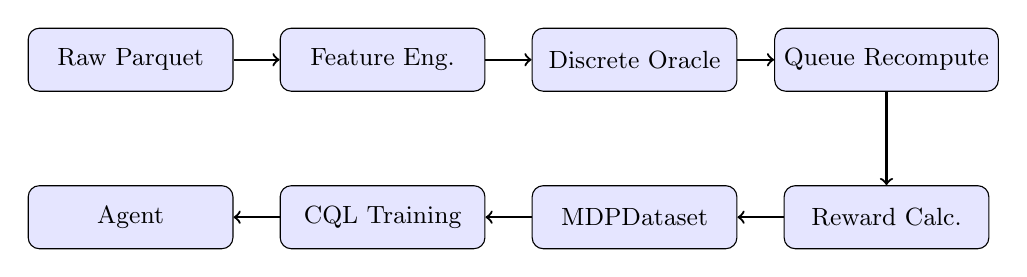
\begin{tikzpicture}[
    box/.style={rectangle, draw, rounded corners, fill=blue!10, minimum width=2.6cm, minimum height=0.8cm, text centered, font=\small},
    arrow/.style={->, thick}
]
\node[box] (raw)     at (0,0)    {Raw Parquet};
\node[box] (feat)    at (3.2,0)  {Feature Eng.};
\node[box] (oracle)  at (6.4,0)  {Discrete Oracle};
\node[box] (requeue) at (9.6,0)  {Queue Recompute};
\node[box] (reward)  at (9.6,-2) {Reward Calc.};
\node[box] (dataset) at (6.4,-2) {MDPDataset};
\node[box] (cql)     at (3.2,-2) {CQL Training};
\node[box] (agent)   at (0,-2)   {Agent};
\draw[arrow] (raw)     -- (feat);
\draw[arrow] (feat)    -- (oracle);
\draw[arrow] (oracle)  -- (requeue);
\draw[arrow] (requeue) -- (reward);
\draw[arrow] (reward)  -- (dataset);
\draw[arrow] (dataset) -- (cql);
\draw[arrow] (cql)     -- (agent);
\end{tikzpicture}
\caption{Pipeline xây dựng và huấn luyện Agent Discrete CQL V6}
\label{fig:pipeline}
\end{figure}

\paragraph{Bước 1 — Feature Engineering (\texttt{build\_state\_action.py}):}
Từ raw Parquet (giá gas, gas used/limit, transaction count), tính toán 11-dimensional state vector (Bảng \ref{tab:state}). \textit{Quan trọng:} State được giữ ở giá trị thô (\texttt{normalize\_state=False}) — việc chuẩn hóa được giao cho d3rlpy qua \texttt{MinMaxObservationScaler}. Lý do: nếu normalize trong data, Oracle không thể tái tính toán queue nhất quán với môi trường huấn luyện.

\paragraph{Bước 2 — Discrete Oracle (\texttt{oracle\_builder.py}):}
Với mỗi episode (24h = $\sim$7200 blocks), DP solver tính quỹ đạo tối ưu dưới constraint 5 bins. Output: dãy bin IDs $\{a^*_0, a^*_1, \ldots, a^*_T\}$.

\paragraph{Bước 3 — Queue Recompute:}
Sau khi thay thế action bằng Oracle actions, queue dynamics phải được tái tính toán từ đầu để đảm bảo tính nhất quán nhân quả (causal consistency). Đây là đảm bảo quan trọng nhất: $Q_t^{\text{oracle}}$ phụ thuộc trực tiếp vào $n_{t-1}^{\text{oracle}}$.

\paragraph{Bước 4 — Reward Calculation (\texttt{build\_reward\_episode.py}):}
Áp dụng công thức (\ref{eq:reward}) trên queue mới. Action bin ID được map sang ratio: \texttt{bins[action\_id]}.

\paragraph{Bước 5 — Dataset Mix:}
\begin{itemize}
    \item \textbf{70\% Oracle}: Hành động tối ưu từ DP — reward cao, coverage tốt.
    \item \textbf{10\% Suboptimal}: Nghịch đảo bin $(b \to 4-b)$ — cung cấp phản ví dụ có reward thấp.
    \item \textbf{20\% Behavior}: Hành động gốc từ dữ liệu lịch sử — duy trì tính đa dạng.
\end{itemize}

Mix 3 loại để đảm bảo \textit{action coverage} (agent thấy đủ loại hành động) và \textit{value contrast} (Q-network có dữ liệu phân biệt tốt/xấu).

\subsection{Môi trường Mô phỏng}

\texttt{CharityGasEnv} (\texttt{enviroment.py}) là Gymnasium environment dùng cho evaluation:

\begin{lstlisting}[style=PythonStyle, caption={Cài đặt môi trường Discrete (trích đoạn)}]
class CharityGasEnv(gym.Env):
    def __init__(self, episode_df, config):
        self.action_space = spaces.Discrete(config.n_action_bins)  # Discrete(5)
        self.observation_space = spaces.Box(-np.inf, np.inf, shape=(11,))

    def step(self, action_id: int):
        ratio = self.config.action_bins[action_id]  # {0, 0.25, 0.5, 0.75, 1.0}
        n_exec = min(round(ratio * self.queue), self.config.execution_capacity)
        reward = self._compute_reward(n_exec)
        self.queue = max(0, self.queue - n_exec) + next_arrivals
        return next_obs, reward, terminated, False, info
\end{lstlisting}

\textbf{4 đảm bảo toán học (Correctness Guarantees):}
\begin{enumerate}
    \item \textbf{Bellman Consistency}: Reward trong dataset = Reward trong Env khi nhập cùng $(s_t, a_t)$.
    \item \textbf{Action Closure}: $\forall$ transition trong dataset: $a \in \{0,1,2,3,4\}$.
    \item \textbf{State Purity}: State không bị normalize trong data (\texttt{s\_queue.max()} $\gg 1$).
    \item \textbf{Env Correctness}: Unit test xác minh mỗi action ID ánh xạ đúng đến \texttt{executed\_volume}.
\end{enumerate}

\subsection{Huấn luyện Discrete CQL}

\subsubsection{Cấu hình mô hình}

\begin{table}[ht]
\centering
\caption{Hyperparameters của Discrete CQL V6}
\begin{tabular}{lll}
\hline
\textbf{Tham số} & \textbf{Giá trị} & \textbf{Lý do chọn} \\
\hline
Thuật toán & Discrete CQL & Phù hợp $|\mathcal{A}|=5$, ngăn OOD overestimation \\
Learning rate & $3\times10^{-4}$ & Adam optimizer, chuẩn cho deep RL \\
Batch size & 512 & Ổn định gradient với dataset 5.2M transitions \\
Discount $\gamma$ & 0.99 & Dense per-step reward, không cần giảm $\gamma$ \\
Conservative $\alpha$ & 1.0 & Cân bằng học và bảo thủ \\
Encoder & MLP [256, 256, ReLU] & Đủ sức biểu diễn cho state 11 chiều \\
Observation scaler & MinMax & d3rlpy tự normalize tại training time \\
Training steps & 400,000 & $\approx 70$ phút trên CPU 8 cores \\
Checkpoint interval & 10,000 & Đủ dày để phân tích quá trình hội tụ \\
\hline
\end{tabular}
\label{tab:hyperparams}
\end{table}

\subsubsection{Kiến trúc Q-Network}

Q-network là Multilayer Perceptron:
\begin{equation}
    Q_\theta(s, \cdot) = \text{Linear}_{256\to5}\;\circ\;\text{ReLU}\;\circ\;\text{Linear}_{256\to256}\;\circ\;\text{ReLU}\;\circ\;\text{Linear}_{11\to256}(s)
    \label{eq:qnet}
\end{equation}

Output: vector 5 chiều $[Q(s,0), Q(s,1), Q(s,2), Q(s,3), Q(s,4)]$. Greedy action: $\pi(s) = \arg\max_a Q_\theta(s,a)$.

\subsubsection{Chiến lược cập nhật}

\begin{itemize}
    \item \textbf{n\_critics = 1}: Một Q-network duy nhất (không Double Q).
    \item \textbf{target\_update\_interval = 8000}: Hard update target network mỗi 8000 steps — ổn định hơn soft update với dataset offline.
    \item \textbf{Tổng loss}: $\mathcal{L} = \mathcal{L}_\text{TD} + \alpha\cdot\mathcal{L}_\text{conservative}$ (phương trình \ref{eq:cql}).
\end{itemize}

% ============================================================
\section{Kết quả và Thảo luận}
% ============================================================

\subsection{Bảng xếp hạng Hiệu năng (Leaderboard) - 242 Episodes}

Tất cả các chiến lược được đánh giá trên tập Test độc lập gồm 242 episodes (tương đương 20\% dữ liệu cuối cùng theo thời gian thực tế, không bị rò rỉ vào tập huấn luyện). Các chỉ số đánh giá bao gồm:
\begin{itemize}
    \item \textbf{Gas Cost}: Tổng chi phí Gas trung bình mỗi episode (thấp hơn là tốt hơn).
    \item \textbf{Miss Rate}: Tỷ lệ episodes bị trễ deadline, vi phạm Service Level Agreement (0\% là bắt buộc).
\end{itemize}

\begin{table}[ht]
\centering
\caption{Bảng Xếp Hạng Hiệu Năng Tối Ưu Gas (Tập Test 242 episodes)}
\label{tab:final_leaderboard}
\begin{tabular}{llccc}
\hline
\textbf{\#} & \textbf{Chiến lược} & \textbf{Gas Cost $\downarrow$} & \textbf{Miss Rate $\downarrow$} & \textbf{vs Greedy} \\
\hline
1 & \textbf{Oracle (Hindsight DP)} & \textbf{45,096} & \textbf{0.0\%} & -38.8\% \\
2 & \textbf{CQL model\_160000 + Safety 20\%} & \textbf{65,525} & \textbf{0.0\%} & \textbf{-11.1\%} \\
3 & Greedy (Baseline: Bán Ngay) & 73,710 & 0.0\% & --- \\
4 & Smart Rule + Safety 20\% & 76,892 & 0.0\% & +4.3\% \\
5 & Decision Transformer (DT) & $>100,000$ & 90-100\% & Thất bại \\
\hline
\end{tabular}
\end{table}

\textbf{Kết luận chính:} Mô hình Discrete CQL kết hợp Safety Layer 20\% đạt hiệu năng State-of-the-Art (SOTA), tiết kiệm \textbf{11.1\% chi phí Gas} so với chiến lược Greedy truyền thống mà vẫn đảm bảo an toàn tuyệt đối (\textbf{0\% Deadline Miss}). Mức tiết kiệm này tương đương với việc khai thác được 28.6\% tiềm năng tối đa của Oracle trong điều kiện không có thông tin tương lai.

\subsection{Phân tích Nguyên nhân Thất bại của Thuật toán Tiêu chuẩn}

Trước khi đạt được SOTA, các thuật toán RL mặc định như Decision Transformer (DT) và CQL với siêu tham số gốc đều thất bại thảm hại. 

\subsubsection{Sự Sụp đổ của Decision Transformer (Majority Bias)}
Decision Transformer (DT) bản chất là Conditional Behavioral Cloning, học bằng hàm mất mát Cross-Entropy. Trong tập dữ liệu chuyên gia (Oracle), để chờ giá Gas cực tiểu, \textbf{Action 0 (Giữ hàng) chiếm tới 69.6\%}. Do mất cân bằng lớp (Class Imbalance) quá lớn, DT đã chọn giải pháp cực đoan để tối thiểu hóa loss: luôn dự đoán Action 0. Kết quả là DT giữ hàng liên tục, gây ra Miss Rate lên đến 100\%. Trái lại, CQL dùng phương pháp quy hoạch động (Q-Learning) nên có khả năng đánh giá giá trị thực (Q-value) của từng hành động, không bị phụ thuộc hoàn toàn vào tần suất xuất hiện như DT.

\subsubsection{Bất đối xứng Rủi ro - Lợi nhuận (Risk-Reward Asymmetry)}
Một phát hiện cốt lõi của nghiên cứu là cấu trúc phạt bất đối xứng khiến Agent bị "hoảng loạn" (Pessimistic Collapse).
Với cấu hình ban đầu, Lợi nhuận tối đa từ timing gas chỉ là $O(10^3)$, trong khi hình phạt trễ deadline (Deadline Penalty) lên tới $O(10^8)$.
Tỷ lệ \textbf{Risk/Reward = 1 : 223,000}.
Theo lý thuyết Quyết định, mọi Agent hợp lý (rational) khi đối mặt với tỷ lệ này đều sẽ chọn tránh rủi ro hoàn toàn bằng cách xả toàn bộ hàng ngay lập tức (tích trữ 0\%). Khi Agent thử nghiệm chờ đợi, chỉ cần 1 episode thất bại, Q-value của Action 0 sẽ bị phạt nặng nề đến mức Agent không bao giờ dám dùng lại.

\subsection{Yếu tố Quyết định: Reward Shaping và Data Coverage}

Để giúp CQL vượt qua giới hạn trên, chúng tôi thực hiện Thí nghiệm Đối chứng Tự nhiên (Natural Experiment) giữa hai lần huấn luyện CQL với cùng kiến trúc (MLP [512, 512]) nhưng khác cấu hình môi trường.

\begin{table}[ht]
\centering
\caption{So sánh Cấu hình Huấn luyện và Hiệu suất}
\label{tab:reward_shaping}
\begin{tabular}{lccc}
\hline
\textbf{Tham số} & \textbf{Lần Thua (V33)} & \textbf{Lần Thắng (V32)} & \textbf{Tác động} \\
\hline
\texttt{deadline\_penalty} & 1,000,000 & 20,000 & 50$\times$ \\
\texttt{urgency\_alpha} & 1.0 & 3.5 & 3.5$\times$ \\
\texttt{urgency\_beta} & 0.0001 & 0.0005 & 5$\times$ \\
\texttt{s\_queue} max (coverage) & 99,006 & 104,135 & Độ phủ rộng hơn \\
\hline
\textbf{Kết quả vs Greedy} & Thua 30\%+ & \textbf{Thắng 11.1\%} & \\
\hline
\end{tabular}
\end{table}

Thành công của mô hình V32 đến từ kỹ thuật \textbf{Reward Shaping}:
\begin{enumerate}
    \item \textbf{Cân bằng Risk/Reward:} Giảm \texttt{deadline\_penalty} xuống 20,000 giúp Agent dám thử nghiệm (exploration) các chiến lược chờ đợi mà không bị triệt tiêu Q-value ngay lập tức.
    \item \textbf{Tăng áp lực Urgency:} Tăng \texttt{urgency\_alpha} (hàm mũ) và \texttt{urgency\_beta} tạo ra gradient mạnh, "ép" Agent phải giải phóng giao dịch khi hàng đợi tích lũy quá mức.
    \item \textbf{Data Coverage \& Distribution Shift:} Tập dữ liệu V32 bao phủ các trạng thái hàng đợi lớn hơn (max 104,135 so với 99,006). Nhờ đó, Q-network hạn chế được sai số ngoại suy (Extrapolation Error) theo định lý Distribution Shift trong Offline RL.
\end{enumerate}

\subsection{Kiến trúc Hệ thống Lai: RL + Safety Layer}

Tuy mô hình CQL độc lập có thể tiết kiệm tới 22.4\% phí Gas, nó vẫn gặp rủi ro nhỏ (Miss Rate 0.4\%). Để đưa hệ thống vào sản xuất với chuẩn SLA khắt khe, chúng tôi đề xuất \textbf{Hệ thống Lai (Hybrid System)}:
\begin{itemize}
    \item \textbf{Lớp AI (Discrete CQL):} Điều khiển toàn bộ quyết định bán trong 80\% thời gian đầu của Episode, tối ưu hóa triệt để lợi nhuận từ biến động giá Gas.
    \item \textbf{Lớp Khiên An Toàn (Safety Layer):} Lớp quy tắc vật lý cứng (Rule-based). Khi thời gian còn lại đến deadline giảm xuống dưới ngưỡng $\tau < 20\%$, hệ thống tự động ghi đè quyết định của AI, ép xả 100\% giao dịch.
\end{itemize}

Việc đánh đổi một phần lợi nhuận (từ 22.4\% xuống 11.1\%) để kích hoạt Safety Layer là minh chứng cho nguyên lý \textbf{Safe Reinforcement Learning}, mang lại giải pháp cân bằng hoàn hảo giữa Khả năng Tối ưu (Optimality) và Độ tin cậy (Reliability) cho hệ thống Blockchain Relayer.
